\documentclass{beamer}

\usepackage{graphicx}

\usecolortheme[named=blue]{structure}

\mode<presentation>
{
  \usetheme{Warsaw}
  \setbeamercovered{transparent}
  \setbeamertemplate{items}[ball]
  \setbeamertemplate{theorems}[numbered]
  \setbeamertemplate{footline}[frame number]
  
% custom colors
  \setbeamercolor{structure}{fg=red!90!black}
  
  \setbeamerfont{section number projected}{%
  	family=\rmfamily,series=\bfseries,size=\normalsize
  }
  \setbeamercolor{section number projected}{bg=red,fg=white}
  \setbeamercolor{frametitle in head}{fg=Brown,bg=Brown!20}
  
}

% \usecolortheme{spruce}

\usepackage{beamerthemesplit}
\usepackage{graphics}
\usepackage{graphicx}
\usepackage{hyperref}
\usepackage{color}
\usepackage{listings}
\usepackage[utf8]{inputenc}

\newcommand{\code}[1]{\texttt{\small{#1}}}
\hypersetup{%
  colorlinks=true,
  urlcolor=red,
  linkcolor=red,
  pdfborderstyle={/S/U/W 1}
}

\definecolor{javared}{rgb}{0.6,0,0} % for strings
\definecolor{javagreen}{rgb}{0.25,0.5,0.35} % comments
\definecolor{javapurple}{rgb}{0.5,0,0.35} % keywords
\definecolor{javadocblue}{rgb}{0.25,0.35,0.75} % javadoc

\lstdefinelanguage{scala}{
  morekeywords={abstract,case,catch,class,def,%
    do,else,extends,false,final,finally,%
    for,if,implicit,import,match,mixin,%
    new,null,object,override,package,%
    private,protected,requires,return,sealed,%
    super,this,throw,trait,true,try,%
    type,val,var,while,with,yield},
  otherkeywords={=>,<-,<\%,<:,>:,\#,@,>,<},
  sensitive=true,
  morecomment=[l]{//},
  morecomment=[n]{/*}{*/},
  morestring=[b]",
  morestring=[b]',
  morestring=[b]"""
}
\lstset{
%   frame=tb,
  language=Scala,
  aboveskip=3mm,
  belowskip=3mm,
  columns=flexible,
  basicstyle=\ttfamily\small,
  keywordstyle=\color{javapurple}\bfseries,
  stringstyle=\color{javared},
  commentstyle=\color{javagreen},
  morecomment=[s][\color{javadocblue}]{/**}{*/},
  numbers=none,
  numberstyle=\tiny\color{black},
  stepnumber=2,
  numbersep=10pt,
  showspaces=false,
  showstringspaces=false,
  tabsize=4
}

\newcommand{\screenshot}[1]{\centerline{%
    \includegraphics[height=7.8cm,transparent]{#1}}}  % 7.8in

\title
  [Wollok: relearning how to teach OOP]
  {Wollok: relearning how to teach Object-Oriented Programming}
\author[Passerini, Fernandes, Tesone]{%
  Javier Fernandes\inst{1,2} \and
  Nicolás Passerini\inst{1,2,4} \\
  Pablo Tesone\inst{3,1,2,4} \and
  Débora Fortini\inst{1,4} \\
  Nahuel Palumbo\inst{4} \and
  Juan Contardo\inst{4} \and
  Carlos Raffellini\inst{4}
}  

\institute{
  \inst{1}Universidad Nacional de Quilmes \\
  \inst{2}Universidad Nacional de San Martin \\
  \inst{3}Universidad Nacional del Oeste \\
  \inst{4}Universidad Tecnológica Nacional - F.R. Buenos Aires.
}

\date{\small Dec 1, 2015}
% \date[WISIT 2015]{\small Workshop de Ingeniería en Sistemas y Tecnologías de la Información \\ 19/09/2015}
\subject{Computational Sciences}

%\logo{\includegraphics[height=1.0cm]{fsu_logo.pdf}}

\begin{document}
  \frame
  {
    \titlepage
  }

  \frame
  {
    \frametitle{Agenda}
    \tableofcontents
  }

\section{Intro}
\subsection{Context}
\frame{
	\frametitle{Context: what do we do}
	\begin{itemize}
	    \item We teach object-oriented programming
	    \item Most of the time in engineering careers
	    \begin{itemize}
	    		\item i.e. people who are supposed to produce industrial software	    
	    		\item and have little previous (structured) programming experience
	    \end{itemize}
	    \medskip
	    \item Planning to translate this experience to highschools in 2016
	    \item Some experience working with smaller kids
	    \\\pause ...but is not what we plan to talk about today
	\end{itemize}
}

\frame{
	\frametitle{Context: what we try to solve}
	\begin{itemize}
		\item Low approval rates
		\item Bad programming practices enforced
		\item Low understanding of the fundamental concepts
		\item Low quality of software produced
	\end{itemize}
	\pause
	\bigskip
	Why is that?
	\begin{itemize}
		\item Low abstraction capabilities
		\item Little mathematical background
		\item And also behavioral issues
		\begin{itemize}
			\item Lack of concentration
			\item High abandonment rates
		\end{itemize}
	\end{itemize}
	
}

\subsection{Why is it so difficult to learn OOP?}
\defverbatim[colored]\helloWorldJava{
\begin{lstlisting}[language=Java]
		package examples;
		
		public class HelloWorld {
			public static void main(String[] args) {
				System.out.println("Hello World");
			}
		}
\end{lstlisting}
}

\frame{
	\frametitle{Introducción}
	\framesubtitle{Why is it so difficult to learn OOP?}	
	\begin{itemize}
    \item Focus on a particular language
    \item Too much concepts to be learnt
    \medskip
    \helloWorldJava
    \pause
    \item Limited or inadequate \textbf{development environments}
    \item To learn programming demands to \textbf{create and handle abstractions}
	\end{itemize}
}

\subsection{Influences \& Previous Work}
\frame{
	\frametitle{Introduction}
	\framesubtitle{Influences and previous work}
	
\includegraphics[width=9pt,height=9pt,natwidth=66pt,natheight=50pt]{images/ozono-icon.png}
	\textbf{Ozono} \hfill \texttt{\footnotesize
	\href{http://ozono.uqbar-project.org/}{http://ozono.uqbar-project.org/}}
	\begin{itemize}
		\item Based on Pharo Smalltalk
		\begin{itemize}
			\item Image-based
			\item Dynamic language
		\end{itemize}
		\item \textbf{Incremental learning path}\footnote{Lombardi, Passerini and Cesario, FRBA, 2007}
	\end{itemize}
	
	\pause\bigskip
	
\includegraphics[width=9pt,
			 	height=9pt,natwidth=313pt,natheight=365pt]{images/gobstones-icon.png}
	\textbf{Gobstones} \hfill \texttt{\footnotesize
	\href{http://www.gobstones.org/}{http://www.gobstones.org/}}
	\begin{itemize}
		\item Careful selection of syntactic elements
		\item No need of input/output
		\item Separation of pure and effectful elements
	\end{itemize}
}

\subsection{A little bit of history: Ozono}
\frame{
	\frametitle{Our first proposal}
	\begin{enumerate}
		\item Think about the learning path
		\begin{itemize}
			\item Introduce concepts gradually
			\item Start with fundamental ones:
				\\\hspace{2em} object - message - references - polymorphism
			\item Postpone others: 
				\\\hspace{2em} classes - inheritance - ...
		\end{itemize}

		\pause
		\medskip
		\item Build a customized tool
		\begin{itemize}
			\item Programming language
			\item Development environment			
			\item Visualization tools
			\begin{itemize}
				\item (Dynamic) object diagram
				\item (Static) class diagram
			\end{itemize}
		\end{itemize}
	\end{enumerate}
}

\frame{
	\frametitle{After seven years of learning...}	
	Ozono was a succesful idea:
	\begin{itemize}
		\item Approval rates raised (from 40 - 50\% to 80 - 90\%)
		\item Exported to other universities: UNQ, UNSAM, UNO, FRD, ...
		\item Big community ($>$ 30 teachers and/or developers)
		\item Research projects
	\end{itemize}

	\bigskip
	But...
}

\frame{
	\frametitle{After seven years of learning...}	
	\begin{itemize}
		\item Lacks a transition from object-based to class-based
		\pause
		\item Environment shortcommings
			\begin{itemize}
				\item Very attached to Pharo (Eg. debugger)
				\item Some tools are not suited for learning
			\end{itemize}
		\pause
		\item Sometimes we miss static type information
			\begin{itemize}
				\item Some simple errors are difficult to detect
				\item It is more difficult to guide the programmer
			\end{itemize}
		\pause
		\item Far from \emph{mainstream} languages
			\begin{itemize}
				\item Image-baed
				\item Unsuitable for some industrial tools (eg. github)
			\end{itemize}
	\end{itemize}
}

\section{Our new proposal: Wollok}
\frame{
	\frametitle{Wollok}
	\framesubtitle{The big picture}
	\begin{itemize}
		\item Methodology: incremental learning path
			\begin{itemize}
				\item Additive meta-model
				\item Progressive examples \& exercises
			\end{itemize}
		\item Language + IDE (+ lots of related tools)
		\item Optimized for teaching \\
			but close to their \emph{mainstream} industrial counterparts!
		\item Empower the students to use the best development practices
		\item Integrated assignment submission, correction and grading (starting)
	\end{itemize}
}

\subsection{Introduction}
\frame{
	\frametitle{Wollok the methodology}	
	\framesubtitle{Incremental learning path}
	
	\begin{center}
		\begin{figure}
			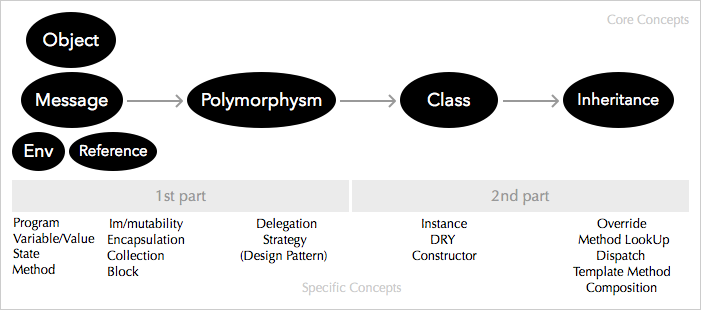
\includegraphics[height=0.65\textheight,natwidth=701,natheight=310]{images/wollok-learning-path.png}
		\end{figure}
	\end{center}	
}

\frame{
	\frametitle{Wollok the language}	
	\framesubtitle{Emphasize the programming concepts}
	\begin{itemize}
		\item Combines \emph{object-based} with class-based programming
	 	\item Everything is an object
	 	\item \emph{Almost} everything is done through messages
	 		\footnote{We have if and try/catch constructs.}
	    \item \emph{Educative} syntax (eg: method \& inherits keywords)
	    \item Selected concepts (eg: differentiate val vs. var)
		\item \emph{Pluggable} type system (in progress)
	\end{itemize}
}

\frame{
	\frametitle{Wollok the language (+ tools)}
	\framesubtitle{Warning: Do not miss the evolution of industrial tools!}
	\begin{itemize}
		\item Light and \emph{modern} syntax \\
			{\footnotesize Eg. lambdas, literals, exceptions, constructors}
		\item Mixins (planned)
		\item Ad-hoc testing constructs
		\\
		\item File-based object environment
		\item Simplified code repository integration (starting)
	\end{itemize}
}

\subsection{Discussion}
\frame{
	\frametitle{Discussion: Why a new language?}
	Because it allows for 100\% customization.
	\pause
	\begin{itemize}
		\small
		\item Better error detection (eg: mandatory return)
		\item Avoid overloaded APIs (eg: collections)
		\item Integrated tools
	\end{itemize}
	
	\pause
	\medskip
	Additive meta-model
	\begin{itemize}
		\small
		\item Start only with objects
		\item Add classes playing nicely with preexisting programs
		\item Another example: import system
	\end{itemize}
}

\frame{
	\frametitle{Some details}	
	\begin{itemize}
		\item Explicit receiver, always write obj.msg()
		\item Many literal objects: collections, positions, date \& time (planned)
		\item Initial values for variables \& constants
		\item Objects can inherit from classes
		\item Operator precedence
		\item Abreviated syntax for mathematical assignments $a += 10$
	\end{itemize}
}

\frame{
	\frametitle{More discussions...}	
	\begin{itemize}
		\item Standalone objects are visible globally
		\item \emph{Impure} language
		\begin{itemize}
			\item If construct 
			\item Try/catch construct	
			\item Constructors
		\end{itemize}
		\item Image vs. file based
		\bigskip
		\item Why not have properties?
		\item Object literals $=>$ a class-less way of code sharing?
	\end{itemize}
}

\subsection{Advanced IDE features}

\frame{
	\frametitle{Advanced features}	
	\begin{itemize}
	    \item Debugger
	    \item Automatic class \& object diagrams
	    \item Integrated testing framework
	    \item Navigation (eg: go to the definition)
		% \item Sensitive searches (ej: referencias, implementaciones, usos)
	    \item Content assist, autocomplete
	    \item Quick fixes
	    \item Automatic refactorings (in progress)
	    \item I18N
		\item Wizards / templates (eg. create project/class/object/test)
	    \item Integrated groupware (in progress)
	    \\
	    \item Integration in other editors (sublime, ace)
	    \item Configurable syntax (prototypes)
	\end{itemize}
}

\frame{
	\frametitle{Advanced Features}
	\framesubtitle{Debugger}
	\begin{itemize}
	    \item Integrated to Eclipse Debugger
	    \item Breakpoints
	    \item Step, into, out 
	    \item Inspect variables
	    \item Object diagram
	\end{itemize}
}

\frame{
	\frametitle{Advanced Features}
	\framesubtitle{Unit testing}
	\begin{center}
		\begin{figure}
			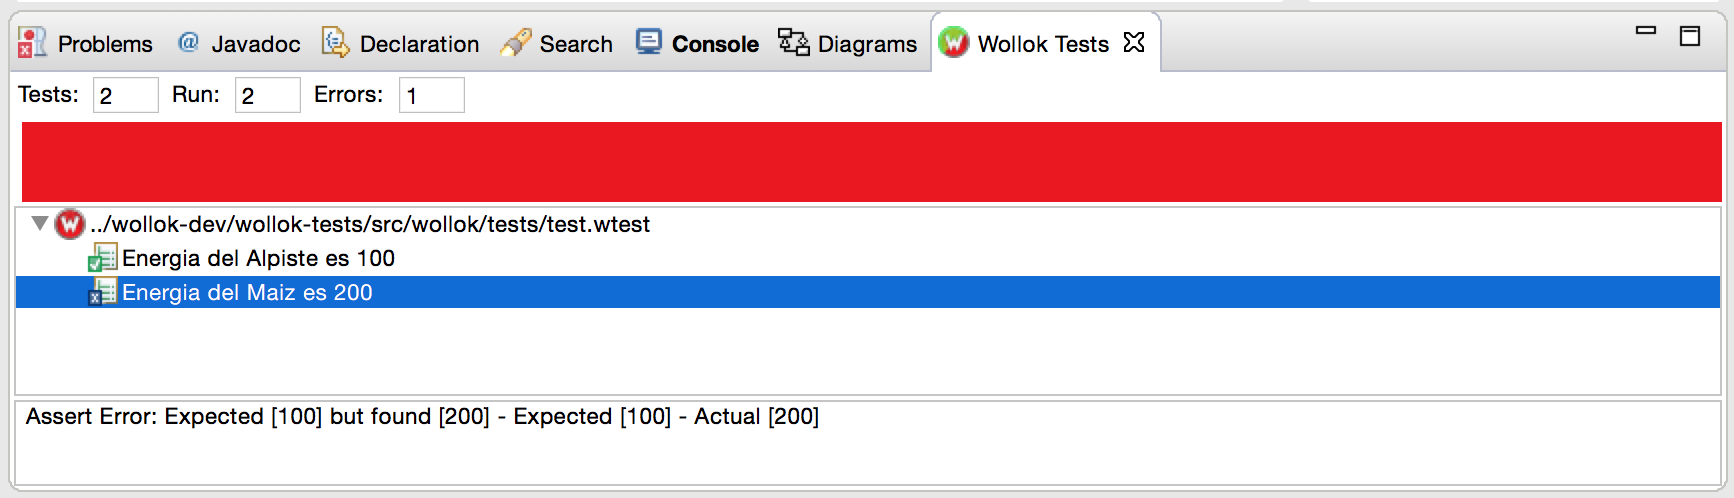
\includegraphics[width=1\textwidth,natwidth=1734,natheight=498]{images/tests.png}
		\end{figure}
	\end{center}
}

\frame{
	\frametitle{Advanced Features}
	\framesubtitle{Sublime editor support}
	\begin{itemize}
	    \item WDK
	    	\begin{itemize}
	    		\item No IDE
	    		\item $\sim70$MB (vs $\sim140$)
	    		\item Headless: wchecker, winterpreter, wtest
	    	\end{itemize}
	    \item Syntax highlight
	    \item Templates 
	    \item Linter
	\end{itemize}
}


\frame{
	\frametitle{Sublime Support}
	\framesubtitle{Syntax Highlight}	
	\begin{center}
		\begin{figure}
			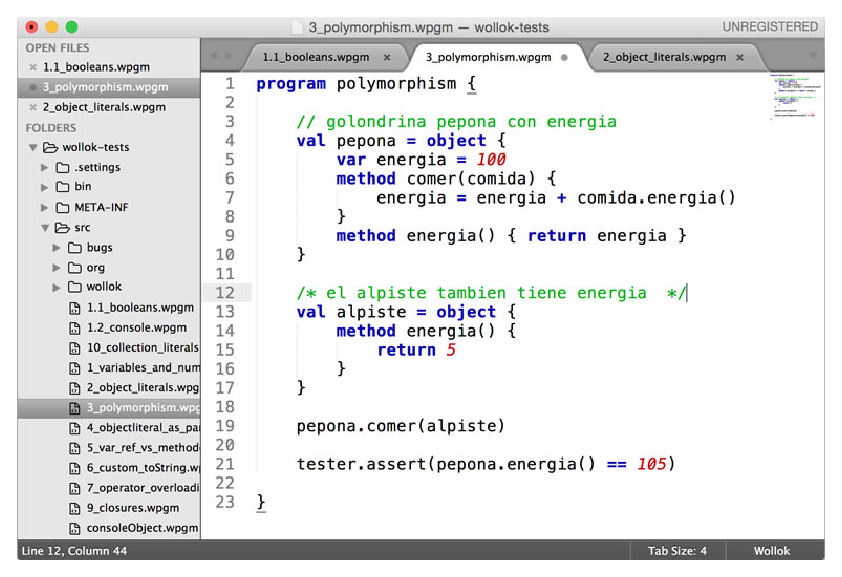
\includegraphics[height=0.8\textheight,natwidth=800,natheight=561]{images/wollok-wisit-sublime-syntax.eps}
		\end{figure}
	\end{center}
}

\frame{
	\frametitle{Sublime Support}
	\framesubtitle{Linter}
	\begin{center}
		\begin{figure}
			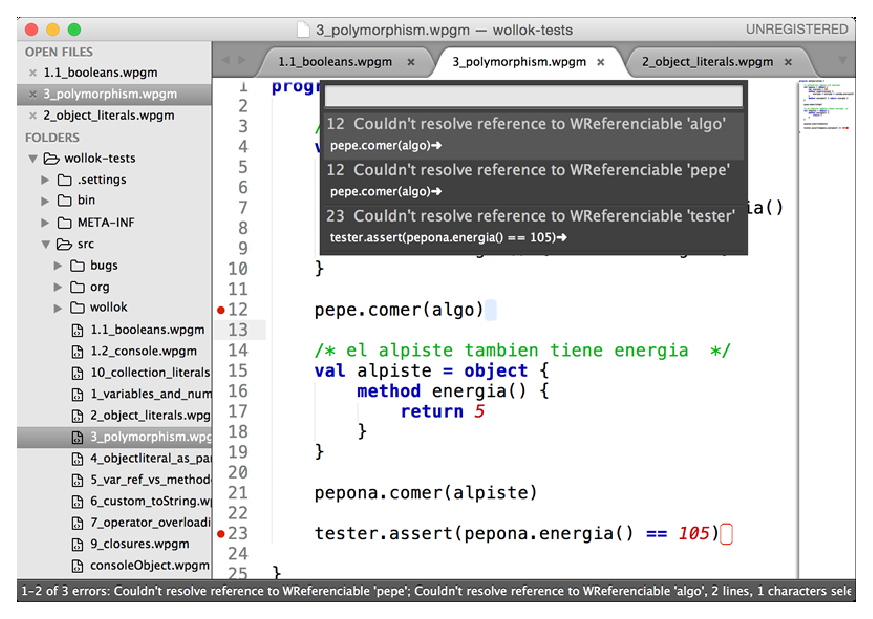
\includegraphics[height=0.8\textheight,natwidth=800,natheight=558]{images/wollok-wisit-sublime-linter.eps}
		\end{figure}
	\end{center}
}


%
% WOLLOK GAME
%

\subsection{Wollok Game}
\frame{
	\frametitle{Wollok Game}
	\begin{itemize}
		\item Herramienta complementaria al testeo unitario y consola interactiva.
		\item Mejorar la comprensión de conceptos.
		\item Visualización de comportamiento
		\item Motivación en el aprendizaje fomentando la participación.
	\end{itemize}
}

\frame{
	\frametitle{Wollok Game}
	\framesubtitle{FarmVille}
	\textbf{FarmVille} - Demo
	
	\begin{center}
		\begin{figure}
			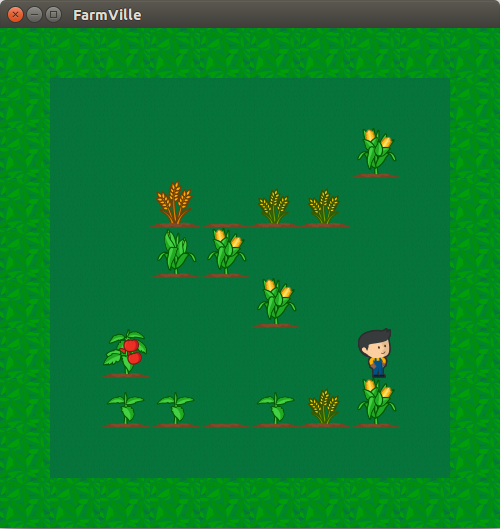
\includegraphics[width=0.4\textwidth,height=0.6\textheight,natwidth=500,natheight=529]{images/wollok-game-farmville.png}
		\end{figure}
	\end{center}
}

\frame{
	\frametitle{Wollok Game}
	\framesubtitle{Sokoban}
	\textbf{Sokoban} - Demo
	
	\begin{center}
		\begin{figure}
			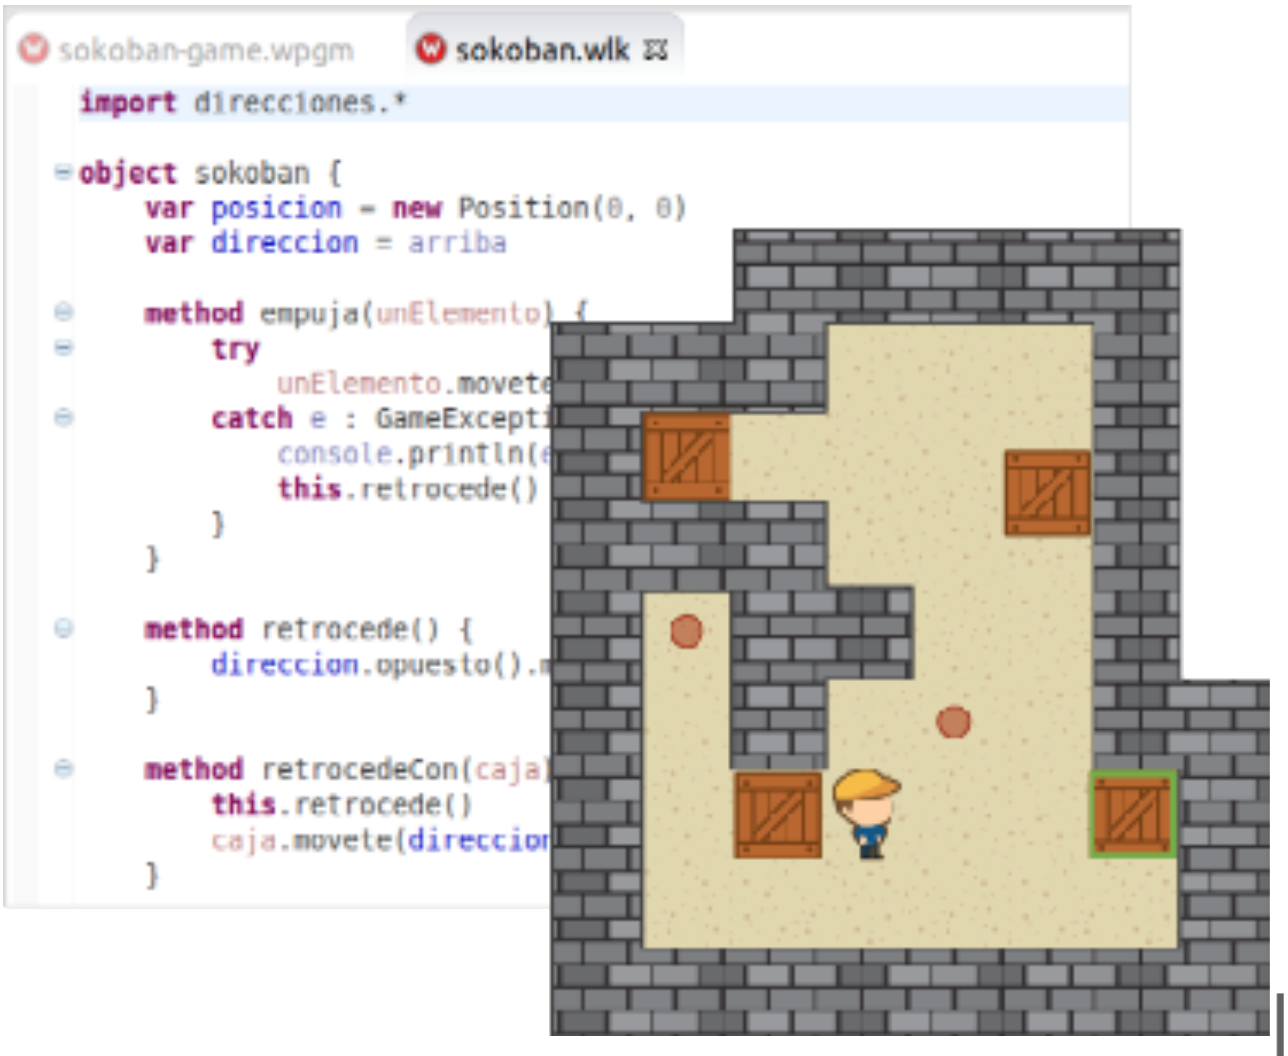
\includegraphics[width=0.4\textwidth,height=0.6\textheight,natwidth=258,natheight=289]{images/wollok-game-sokoban.png}
		\end{figure}
	\end{center}
}

\frame{
	\frametitle{Wollok Game}
	\framesubtitle{Future work}
	\begin{itemize}
		\item More types of \textbf{Games}
		\begin{itemize}
		  \item Survival
		  \item Turn-based
		\end{itemize}
		\item More types of \textbf{Interactions}
		\item Visual features
		\begin{itemize}
		  \item Animations
		  \item Infinite backgrounds
		  \item Different view (side view, isometric view, ...)
		\end{itemize}
	\end{itemize}
}

\section{Under the hood}
\frame{
	\frametitle{Wollok development}	
	\begin{itemize}
		\item OpenSource: LGPLv3 
		\item Stack: 
\includegraphics[width=9pt,
			 	height=9pt,natwidth=32,natheight=32]{images/eclipse-icon.png} Eclipse XText +
			 	Xtend Lang
		\item SCM:
			\begin{itemize}
			  	\item \textbf{Code}: 
\includegraphics[width=9pt,
			 	height=9pt,natwidth=16pt,natheight=16pt]{images/github-icon.png} GitHub
			  	(\href{https://github.com/uqbar-project/wollok}{uqbar-project/wollok})
			 	\item \textbf{Build}: Maven + Tycho
			 	\item \textbf{Continuous Integration}:
			 	
\includegraphics[width=9pt,
			 	height=9pt,natwidth=50pt,natheight=50pt]{images/travis-ci-icon.png} Travis
			 	\item \textbf{Continuous Deployment}
			 	\item \textbf{Coverage}: coveralls + jacoco
			 \end{itemize}
		\item Testing \& TDD
	\end{itemize}
}

\frame{
	\frametitle{Wollok development}
	\framesubtitle{Continuous Integration \& Deployment}	
	\begin{itemize}
	  	\item \textbf{GitFlow}
	  		\begin{itemize}
	  		  \item Feature Branches
	  		  \item Pull-Requests
	  		  \item $dev \rightarrow master \leftarrow  hotfixes$ 
			\end{itemize}	 
		\item \textbf{Integration}:
			\begin{itemize}
			  \item Travis
			  \item compile, test, coverage, deploy
			\end{itemize}
		\item Deployment:
				\begin{itemize}
				  \item \textbf{Products} (IDE): multiple platforms
				  \item \textbf{Update Sites}
				  \item \textbf{WDK}
				  \item 2 Environments: Stable \& Dev
				\end{itemize}
	\end{itemize}
}

\frame{
	\frametitle{Wollok Development}
	\framesubtitle{Testing \& TDD}	
	\begin{itemize}
	  	\item 87\% coverage
	  	\item \textbf{Runtime}      % SCREEN: ACA MOSTRAMOS UN SCREENSHOT DE UN TEST
	  		\begin{itemize}
	  		  \item Test program execution
	  		  \item Interpreter
	  		  \item \textbf{JUnit + iDSL}
			\end{itemize}	 
		\item \textbf{Static}
			\begin{itemize}
			  \item \textbf{Check system}: XPect  % SCREEN: ACA MOSTRAMOS UN TEXT XPECT
			  \item \textbf{Type System}: JUnit + iDSL
			  \item \textbf{Autocomplete}: XPect
			  \item \textbf{Formatting}: JUnit + iDSL
			\end{itemize}
		\item \textbf{Pending}
			\begin{itemize}
			  \item Quick-Fixes
			  \item Refactorings
			\end{itemize}
	\end{itemize}
}

\frame{
	\frametitle{Testing \& TDD}
	\framesubtitle{Runtime}
	Interpreter testing
	\begin{center}
		\begin{figure}
			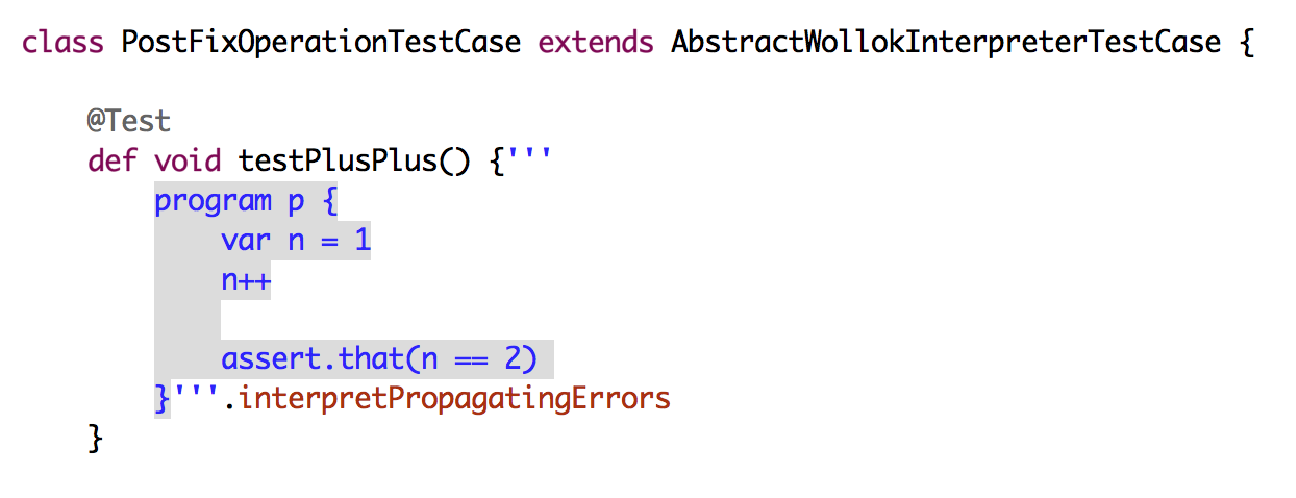
\includegraphics[width=1\textwidth,natwidth=836,natheight=444]{images/wollok-tests-runtime.eps}
		\end{figure}
	\end{center}
}

\frame{
	\frametitle{Testing \& TDD}
	\framesubtitle{Static checks}
	\begin{center}
		\begin{figure}
			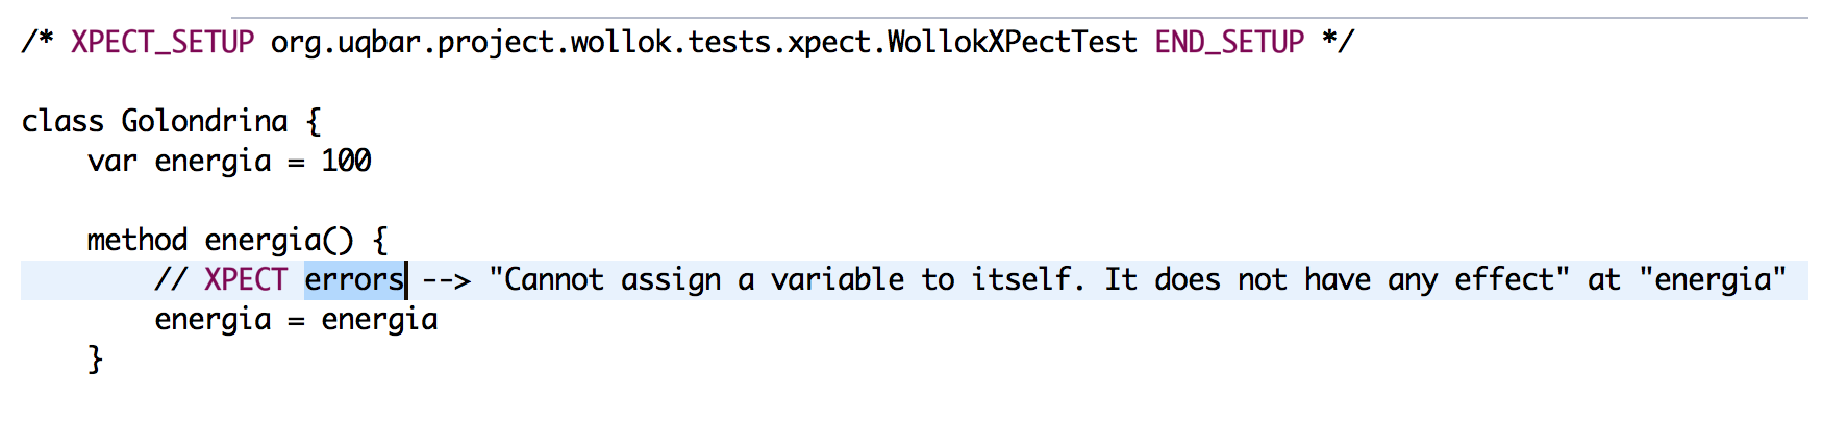
\includegraphics[width=1\textwidth,natwidth=1720,natheight=372]{images/wollok-tests-checkeos.eps}
		\end{figure}
	\end{center}
}

\section{Conclusions \& further work}
\subsection{Teaching experience}
\frame{
	\frametitle{Teaching experience}
	Students intuitively take advantage of the language and tools:
	\begin{itemize}
		\item Class-based + object-based integration
		\item REPL is more intuitive than traditional Smalltalk workspaces
		\item More control over unit testing
		\item More traditional editors
	\end{itemize}
	\pause
	\medskip
	\begin{center}
		An \textbf{incremental learning path} supported by adequate \textbf{tools},\\
		\pause
		empowers students' \textbf{intuition} \\
		\pause
		incrementing their \textbf{autonomy, creativity and motivation}\\
	\end{center}
}

\subsection{Next steps}
\frame{
	\frametitle{Próximos pasos}
	Próximos Pasos
	\begin{itemize}
		\item Varias discusiones sobre la mejor sintaxis (in progress)
		\item Plataforma p/interacción Alumno $ \leftrightarrow $ Docente (starting)
		\item Herencia basada en mixins
		\item Implementar wollok-game en el aula
		\item Block-based editor
	\end{itemize}
	
	Y muchas actividades para sumar más gente al proyecto.
}

\frame{
  \frametitle{Muchas gracias}
  {\LARGE ¡Muchas Gracias!}
  \bigskip
  \begin{center}
		\begin{figure}
			
\includegraphics[width=0.6\textwidth,natwidth=815,natheight=342]{images/logo-fun.png}
		\end{figure}
	\end{center}
}
\end{document}

